% ----------------------------------------------------------------
% achemso --- Support for submissions to American Chemical
%  Society journals
% Maintained by Joseph Wright
% E-mail: joseph.wright@morningstar2.co.uk
% Originally developed by Mats Dahlgren
%  (c) 1996-98 by Mats Dahlgren
%  (c) 2007-2008 Joseph Wright
% Released under the LaTeX Project Public license v1.3c or later
% See http://www.latex-project.org/lppl.txt
% 
% Part of this bundle is derived from cite.sty, to which the
% following license applies:
%   Copyright (C) 1989-2003 by Donald Arseneau
%   These macros may be freely transmitted, reproduced, or
%   modified provided that this notice is left intact.
% ----------------------------------------------------------------
% 
% The achemso bundle provides a LaTeX class file and BibTeX style
% file in accordance with the requirements of the American
% Chemical Society.  The files can be used for any documents, but
% have been carefully designed and tested to be suitable for
% submission to ACS journals.
% 
% The bundle also includes the natmove package.  This package is
% loaded by achemso, and provides automatic moving of superscript
% citations after punctuation.

\documentclass[
%journal=ancac3, % for ACS Nano
%journal=acbcct, % for ACS Chem. Biol.
journal=jacsat, % for undefined journal
manuscript=article]{achemso}
\usepackage[version=3]{mhchem} % Formula subscripts using \ce{}
\usepackage{listings}
\usepackage{amsmath}
\usepackage{titlesec}
\usepackage{setspace}
\usepackage{float}
\restylefloat{table}

\usepackage{natbib}
\bibliographystyle{abbrvnat}
\setcitestyle{numbers,open={(},close={)}}

\usepackage{enumitem}\setlist[description]{font=\textendash\enskip\scshape\bfseries}
\newcommand{\tab}[1]{\hspace{.2\textwidth}\rlap{#1}}
\newcommand*{\mycommand}[1]{\texttt{\emph{#1}}}
\author{Lakshmi Prakash}
\email{lprakash@utexas.edu}
\author{Marek Bejda}
\email{marek.bejda@utexas.edu}
\affiliation[University of Texas at Austin]
{B.S. in Computer Science}


\title[\texttt{achemso} demonstration]
{Performance Analysis for Scaling up R Computations Using Hadoop}



\begin{document}
\vspace{35mm}
\begin{center}
\large
Completed for the Certificate in Statistics and Scientific Computation\\
Spring 2015
\end{center}
\vspace{35mm}

\noindent\rule{7cm}{0.4pt}\\
Dr. Weijia Xu\\
Texas Advanced Computing Center\\
Advisor
\newpage


\lstset{
basicstyle=\small\sffamily,
numbers=left,
numberstyle=\tiny,
frame=tb,
columns=fullflexible,
showstringspaces=false
}



\renewcommand{\abstractname}{Executive Summary}
\begin{abstract}
The number of big data applications in the scientific domain is continuously increasing. R is a popular language among the scientific community and has extensive support for mathematical and statistical analysis. Hadoop has grown into a universally used tool for data manipulation. There are a number of ways of integrating these two tools: Hadoop streaming, RHIPE (R and Hadoop Integrated Programming Environment), and RHadoop. We tested these methods using a basic \textit{wordcount} application. \textit{Wordcount} might not be an all encompassing benchmark, but it provides us with a stable base with very few opportunities for human error. We measured the performance of the three methods on small files, checked their scalability, and tested their effectiveness in handling large files. Of the three options, we found RHIPE to be generally effective, scalable, and consistent, but less customizable. RHadoop tended to be slightly more efficient than R Streaming in performance, yet failed very frequently in our scalability testing. 

\smallskip
\noindent \textbf{Keywords:} \textit{R, big data, Hadoop, Rhipe, RHadoop, Streaming}
\end{abstract}

\newpage
\singlespacing
\tableofcontents
\clearpage

\section{Introduction}
The extensive resources available on the Rustler supercomputer far exceeds the norm but the datasets are growing exponentially; just 6 years ago 100 gigabytes was atypical, now datasets reach terabytes in size. These large datasets drive research around the world. For instance, the NASA spacecrafts monitor everything from our home planet to distant galaxies and send back images and information to Earth. Hundreds of terabytes of data are received every hour; the data needs to be processed to understand Earth and the universe beyond~\citep{JPL}. The computation for research is carried out in a two-step process. First, the datasets are processed using Apache Hadoop, Apache Spark, Presto, or some data processing tool. Then, the data is analyzed using R, Python, or Scala. The performance of this two-step process is both machine and workload dependent. Over the past years, R- a script style programming language has become a popular analytic environment for many domain science fields due to variety of existing scientific packages. We have investigated various solutions of integrating R with Hadoop and evaluated the pros and cons of each approach. We have conducted performance comparison studies for utilizing those approaches, including RHadoop, RHIPE (R and Hadoop Integrated Programming Environment) , and Hadoop streaming on a 48 node cluster. In this paper, we report our performance evaluation results, lessons learned, and recommend best practices when supporting R for big data analysis with high performance resources.    

A recently published paper 'Optimising parallel R correlation matrix calculations on gene expression data using MapReduce' ~\citep{BIO} compared RHIPE performance with a variety of R parallel packages. Concluding that 'The performance evaluation found that the new MapReduce algorithm and its implementation in RHIPE outperforms vanilla R and the conventional parallel algorithms implemented in R Snowfall. We propose that MapReduce framework holds great promise for large molecular data analysis, in particular for high-dimensional genomic data such as that demonstrated in the performance evaluation described in this paper. We aim to use this new algorithm as a basis for optimising high-throughput molecular data correlation calculation for Big Data.'

In 'Big Data Analytics Predicting Risk of Readmissions of Diabetic Patients'~\cite{DIAB} Salian and Dr. Harisekaran use the RHadoop package to analyze data sets searching for a better understanding of the issues that can lead to readmission. Their main emphasis for the RHadoop package was the availability of rhbase which allowed them to use HBase and access their data using sql-like queries. 


\section{Background}
This section provides an overview of R and Python, and the different ways of integrating R with Hadoop, namely RHadoop, RHIPE, and Hadoop Streaming. It also discusses the advantages and disadvantages of each.

\subsection{R}
R is an open source programming language for performing statistical and predictive analysis, data mining and visualization functions on data. R is the most popular language for these purposes. As the data gets large, issues begin to surface because of memory limitations. Large, complex datasets can be structured, semi-structured, or unstructured and typically do not fit into memory. Hence, it is natural to attempt to scale up R computations using Hadoop. 

R has a vast mathematical and statistical package selection on CRAN, which means that many functionalities are readily available for use. The robust supporting community for R in the data industry adds to the convenience. R integrates well with other languages like C++, Java, and C, thereby giving R users great flexibility. R provides extensive native mathematical support. For instance, R's array-oriented syntax makes the translation between math and implementation easier. 

But, the learning curve for R is steep and not very suitable for data with noise. Also, R is slow particularly for non-vectorized code and is slow on Input/Output operations. 

\subsection{Python}
Python, yet another language of choice for the scientific community is geared towards more general programming use. It has numerous packages ranging from web applications and artificial intelligence to 3D modeling and system administration. 

The advantage of Python is that it is very easy language for programmers to learn. It is an object-oriented language, hence it is easier to write large-scale robust code in Python. It is convenient to parse data in python and hence is suitable for data with noise and scrapping purposes. 

Though there are tools like Panda, Numpy, SciPy, etc that help with mathematical and statistical applications, it is still behind R and related support is limited.

\subsection{Hadoop}
Apache Hadoop is an open source Java framework for processing and querying large amounts of data on large clusters of commodity hardware. It is the most commonly used framework for Big Data processing. Two main features of Hadoop are HDFS and mapreduce. 

\subsection{Hadoop Streaming}
Hadoop Streaming enables us to write map and reduce functions in any programming or scripting language that supports reading data from standard input and writing to standard output. This feature makes Hadoop Streaming very flexible and can be easily used by a large number of users. R and Python are two common choices for such a language. We will refer to these two methods as R Streaming and Python Streaming.

There are a lot of parameters that can be customized, for example, number of mappers, number of reducers, jvm memory, input format, output format etc. The default input format for hadoop streaming jobs is TextInputFormat, which reads the data one line at a time.~\cite{Apache}

A well detailed evaluation of Hadoop Streaming given in “More Convenient More Overhead: The Performance Evaluation of Hadoop Streaming”~\cite{Overhead} concluded that the linux pipe() and Java Read/Write calls were the cause of vast overhead in Hadoop streaming. 

\subsection{RHadoop}
RHadoop is a family of R packages that act as a wrapper for Hadoop Streaming and allow the execution of Hadoop jobs without ever leaving the application. It has separate packages \textit{ravro}, \textit{plyrmr}, \textit{rmr}, \textit{rhdfs}, and \textit{rhbase}; the main two components being \textit{rhdfs} and \textit{rmr}. \textit{Rhdfs} is primarily responsible for the handling of HDFS operations such as file manipulation, reading and writing, and directory traversal. \textit{Rmr} is responsible for packaging of the map and reduce functions, hadoop configuration parameters, and the job submission. 

RHadoop is easy to install and setup. It provides support for HBase and Avro. Like R Streaming, there exist numerous customizable parameter options like number of mappers, number of reducers, combiner, vectorized reduce, etc. The version of RHadoop used for testing was 3.3.0.

\subsection{RHIPE}
RHIPE is a single vast package that contains both HDFS and Hadoop management operations. Installation can be a little tricky because of the dependencies, especially Protocol Buffers, but once configured it is very reliable and stable. It is efficient and scales well with data size. It does not depend on the Hadoop streaming jar and comes with a custom inputformat: LApplyInputFormat. LApplyInputFormat allows the file processing to be done chunk wise instead of the default line at a time.  Not using the standard Hadoop streaming however deprives it of certain functionalities, like the ability to swap out input formats. 

A key benefit of RHIPE is the serialization and deserialization of R data structures allowing the user to call 
\begin{lstlisting}
rhcollect(key, [scalar, list, data.frame, matrix]).
\end{lstlisting}
As of version 0.65, RHIPE is capable of serializing scalar vectors such as integers, characters, numerics, logicals, complex, and raw, and lists of scalar vectors and attributes of objects. RHIPE can also serialize data frames, factors, and matrices.~\cite{RHIPEDOCS} With this knowledge, we can easily emit many R data structures and read them in the reducer. 


\section{Methods}
We used the typical \textit{wordcount} program for benchmarking. We ran tests to measure the consistency, scalability, and robustness of each package. Initially we ran tests on a relatively small file with different combinations of mappers and reducers with and without a combiner. We expected to determine the optimal parameters for best performance using the above technique. We then performed scalability testing using the parameters found in the small file tests. Finally, we performed tests on a very large file for the packages that were scalable to test for resource exhaustion. 
The datasets used were downloaded from Google Book N-gram library. ~\cite{GoogleNGram} \\ \\We used the following systems configuration for our tests:
\newline
CentOS 6.5 \\
Cloudera Hadoop Version 5.1.0 \\ 
RHadoop version 3.3.0\\
RHIPE version 0.75\\
R version 3.1.2
\\
Environment configuration:  \\
\begin{lstlisting}[language=bash, caption=\~/.bashrc]
export JAVA_HOME=/usr/lib/jvm/jre-1.7.0-openjdk.x86\_64 
export HADOOP_HOME=/usr/lib/hadoop 
export HADOOP_EXECUTABLE=/usr/bin/hadoop 
export HADOOP_BIN=/usr/lib/hadoop/bin 
export HADOOP=$HADOOP_HOME 
export HADOOP_CONF_DIR=/etc/hadoop/conf 
export HADOOP_EXAMPLES_JAR=/usr/lib/hadoop-mapreduce/hadoop-mapreduce-examples.jar
export HADOOP_STREAMING_JAR=/usr/lib/hadoop-mapreduce/hadoop-streaming.jar 
export HADOOP_STREAMING=$HADOOP_STREAMING_JAR 
export HADOOP_VERSION=hadoop2
export HADOOP_LIBS=/usr/lib/hadoop/client:/usr/lib/hadoop/lib:\
/usr/lib/hadoop:/usr/lib/hadoop-hdfs:/usr/lib/hadoop-yarn:\
/usr/lib/hadoop-mapreduce
\end{lstlisting}

\subsection{Small File Tests}
Dataset used: \\
googlebooks-eng-all-5gram-20120701-un (9.4GB)\\ \\
The goal of the small tests was to quickly determine parameters that work best for the particular file. We started with an estimate of the number of mappers and reducers needed for the file, intentionally erring on the smaller side on both those values ((75, 15) in particular). We then increased the number of mappers keeping the number of reducers constant till a further increase showed no considerable decrease in time taken for the job. The next step was to keep the number of mappers constant at this optimal value, and increase the number of reducers till a further change does not have a considerable effect. The above runs are without using a combiner. We then took the thus found optimal values for the number of mappers and reducers and ran this combination with the combiner. 

The above parameters are the main ones for Python Streaming, R Streaming and RHIPE. But RHadoop has a couple of other parameters that affects performance like in.memory.combine and vectorized.reduce. Both of those can be set to either TRUE or FALSE. We ran tests for all possible configurations of these settings. 

In addition to figuring out the best parameter settings for each package, the purpose of these small tests were to get an idea of how the packages performed relative to each other. 

\subsection{Scalability Tests}
Datasets used: \\
    googlebooks-eng-all-5gram-20120701-un (16.7GB)\\
    googlebooks-eng-all-5gram-20120701-on (25.2GB)\\
    googlebooks-eng-all-5gram-20120701-be (45.7GB)\\
    googlebooks-eng-all-5gram-20120701-in (77.7GB)\\
    googlebooks-eng-all-5gram-20120701-of (104.3GB)\\
    googlebooks-eng-all-5gram-20120701-th (285.1GB)\\ \newline
The goal of these tests was to determine which of the packages could scale up to larger files and how the performance changed with the file size, whether there was a logarithmic, linear, or exponential increase in time taken for the job with a linear increase in file size. These tests give us an estimate for the performance under different workloads. Moreover, these tests are designed to let us conclude on a package that works best in general in terms of performance. 

\subsection{Large File Tests}
Datasets used: \\
    googlebooks-eng-all-5gram-20120701-t*  (390GB)\\
    googlebooks-eng-all-5gram-20120701-*   (700GB)\\ \\
The aim of these is to stress test the packages found to scale well in the Scalability tests, to check if they can handle file sizes of a few hundred Gigabytes.   
    

\subsection{Configuration}    
All three packages offer a number of parameters and configurations that can be tuned to increase performance. For the individual packages these configurations can be adjusted as discussed below.  

\subsubsection{Hadoop Streaming}
\begin{lstlisting}[language=bash, caption=Hadoop streaming]
$ hadoop jar ${HADOOP_STREAMING_JAR}		          \
-Dmapreduce.job.name="Wordcount-book.txt" 		  \
-Dmapreduce.job.maps=100 				   \
-Dmapreduce.job.reduces=20 				   \
-Dmapreduce.map.java.opts=-Xmx11500M 	           	   \
-Dmapreduce.reduce.java.opts=-Xmx11500M 		   \
-files ./mapper.R,./reducer.R  				   \
-mapper ./mapper.R                      		    \
-reducer ./reducer.R		  			    \
-combiner ./reducer.R					    \
-input ./data/book.txt	  				   \
-output ./output/book	  				   \
\end{lstlisting}

We begin the streaming process by calling the hadoop(\textbf{Line 1}) shell script with the jar(\textbf{Line 2}) parameter pointing at the Hadoop Streaming jar (specified by the \\ HADOOP\_STREAMING\_JAR environmental variable). Parameters and behavior of streaming then follow prepended with a -D (\textbf{Line 3}). In the above example \textbf{Lines 2-6} specify the job name, number of mappers, number of reducers, and the amount of memory that should be reserved for the mappers and reducers. 

Once the configuration parameters are set the files to be transfered to the data nodes are specified \textbf{Line 7}, these files can be anything and generally will include the mapper and reducer files, other possibilities include jars, scripts, or text files to be used for caching. \textbf{Lines 8-10} specify the mapper,reducer, and combiner scripts and supply the HDFS input (\textbf{Lines 11-12}) and output paths.

More detailed information on the options available to hadoop streaming can be found on the Apache Hadoop Streaming page ~\cite{Apache} or by running the -info command on the Hadoop Streaming jar.

\begin{lstlisting}[language=bash]
hadoop jar ${HADOOP_STREAMING_JAR} -info

\end{lstlisting}


\subsubsection{RHadoop}

\begin{lstlisting}
bp =
  list(
    hadoop =
      list(
        D = paste("mapred.job.name=", args[[1]], sep=''),
        D = "mapreduce.map.memory.mb=11500",
        D = "mapreduce.reduce.memory.mb=11500",
        D = "mapreduce.map.java.opts=-Xmx11500M",
        D = "mapreduce.reduce.java.opts=-Xmx11500M",
        D = paste("mapreduce.job.maps=", "10" , sep=''),
        D = paste("mapred.reduce.tasks=", "15" , sep='')
  ))

mapreduce(
            input = "hdfs:///book.txt",
            output = "hdfs:///output/book",
            input.format = "text",
            map = wc.map,
            #reduce = wc.reduce, // when vectorized.reduce = F
            reduce = wc.vectorized.reduce, 
            vectorized.reduce = TRUE,
            in.memory.combine = TRUE,
            combine = TRUE
)
\end{lstlisting}
Similarly to the previous hadoop streaming example we begin by specifying the job name, mapper and reducer memory limits, the Java VM memory limits, and mapper and reducers counts. (\textbf{Line 9})
The next block submits the hadoop job using the mapreduce function. Some of the parameters of interest are vectorized.reduce and in.memory.combine. (\textbf{Lines 21-22}) 

\textit{"in.memory.combine- Apply the combiner just after calling the map function, before returning the results to hadoop. This is useful to reduce the amount of I/O and (de)serialization work when combining on small sets of records has any effect (you may want to tune the input format to read more data for each map call together with this approach)"} 

\textit{"vectorized.reduce - The argument to the reduce should be construed as a collection of keys and values associated to them by position (by row when 2-dimensional). Identical keys are consecutive and once a key is present once, all the records associated with that key will be passed to the same reduce call (complete group guarantee). This form of reduce has been introduced mostly for efficiency reasons when processing small reduce groups, because the records are small and few of them are associated with the same key. This option affects the combiner too."}
~\cite{RHADOOP_DOC}

\subsubsection{RHIPE}
\begin{lstlisting}
mapred = list(
        mapred.max.split.size=as.integer(1024*1024*block_size)
        , mapreduce.job.reduces=10
        )
rhipe.results <- rhwatch(
                    map=mapper, reduce=reducer,
                    input=rhfmt("hdfs:///book.txt", type="text"),
                    output="hdfs:///output/book",
                    jobname=paste("rhipe_wordcount_", 1 ,sep="-"),
                    mapred=mapred)
\end{lstlisting}
We create a named list of parameters, specifically \textbf{Line 2} provides the chuck size in bytes and sets the number of reducers \textbf{Line 3}. The job executions \textbf{Line 5} then receives the map and reduce functions \textbf{Line 6}.
RHIPE won't read text documents by default and needs \textbf{Line 7} for conversion we can either specify an output path \textbf{Line 8} or NULL, and finally supply the options (\textbf{Line 9}). 

\section{Results}
The three layer testing proved successful at determining advantages and drawbacks of each package. We were able to determine an order of performance immediately after the first test. The second easily chose RHIPE and Python over RHadoop and R Streaming, both of which proved successful and capable even in the large file tests.

\subsection{Results for Small file tests}
The following are the times for running \textit{wordcount} on a file of around 10GB. We found the optimal reducer to mapper ratio, and the benefits of using a combiner. We saw that Python Streaming was faster than R Streaming; a great performance improvement was achieved in RHadoop by making the code vectorized; RHIPE considerably outbeat other options in R. We also noticed that our choice of R functions to use had a great impact on performance.
\subsubsection{Python Streaming and R Streaming}
\begin{table}[H]
\begin{tabular}{ l | l | l | l }
\# Mappers & \# Reducers & Python Streaming & R Streaming \\ \hline
 75 & 20 & 1mins, 27sec & 6mins, 34sec \\\hline
 86 & 20 & 1mins, 22sec & 7mins, 1sec  \\\hline
 100 & 20 & 1mins, 10sec & 5mins, 39sec  \\\hline
 120 & 20 & 1mins, 3sec & 4mins, 22sec  \\\hline
 100 & 25 & 1mins, 11sec & 5mins, 10sec  \\\hline
 100 & 30 & 1mins, 12sec & 5mins, 12sec  \\\hline
 100 & 35 & 1mins, 15sec & 5mins, 24sec  \\
\end{tabular}
\end{table}
The above table has run times for different numbers of mappers and reducers for Python and R Streaming. It can be seen that Python Streaming is consistently faster than R Streaming. This is because the default input format used by Streaming is TextInputFormat which reads in line by line, and the input-output operations in R are slower than in Python. 

120 mappers and 20 reducers, i.e. a reducer to mapper ratio of 0.17, gave us the lowest time in an average of three runs with the same settings. Also, these times are with the combiner turned on which we found to be faster than the case of not using the combiner for both Python and R Streaming.

\subsubsection{RHadoop}
\begin{table}[H]
\begin{tabular}{ l | l | l | l | l }
\# Mappers & \# Reducers & None & C & C + IMC + VR \\ \hline
 75 & 20 & 11mins, 0sec & 19mins, 52sec & 5mins, 01sec \\\hline
 86 & 20 & 10mins, 36sec & 19mins, 44sec & 4mins, 54sec \\\hline
 100 & 20 & 10mins, 54sec & 18mins, 33sec & 4mins, 4sec \\\hline
 120 & 20 & 11mins, 6sec & 20mins, 3sec & 3mins, 43sec \\\hline
 100 & 25 & 9mins, 46sec & 15mins, 59sec & 4mins, 25sec \\\hline
 100 & 30 & 8mins, 34sec & 15mins, 33sec & 4mins, 17sec \\\hline
 100 & 35 & 7mins, 25sec & 14mins, 19sec & 4mins, 9sec \\
\end{tabular}
\end{table}
In the above table, C stands for combiner, IMC stands for in.memory.combine, and VR stands for vectorized\_reduce. The column headings represent the parameters that were set to TRUE for the corresponding run. 

RHadoop gives a poor performance, it takes almost double the time as R Streaming in the cases without vectorized\_reduce set to true. This is surprising since RHadoop is just a wrapper around R Streaming. But on using vectorized\_reduce, RHadoop actually outbeats R Streaming. 

Another peculiar result with RHadoop is that the runtimes without the combiner is faster than with the combiner when vectorized\_reduce is not used. This is different from what is observed in the Python and R Streaming cases and also in the case of RHIPE as shown below. 
\subsubsection{RHIPE}
\begin{table}[H]
\begin{tabular}{ l | l | l | l }
\# Mappers & \# Reducers & No combiner & With combiner \\ \hline
 75 & 20 & 6mins, 11sec & 2mins, 37sec \\\hline
 86 & 20 & 5mins, 49sec &  2mins, 15sec \\\hline
 100 & 20 & 5mins, 31sec & 2mins, 2sec  \\\hline
 120 & 20 & 5mins, 41sec & 1mins, 47sec  \\\hline
 100 & 25 & 5mins, 48sec & 2mins, 3sec  \\\hline
 100 & 30 & 5mins, 58sec & 2mins, 2sec  \\\hline
 100 & 35 & 6mins, 2sec & 2mins, 6sec  \\
\end{tabular}
\end{table}
RHIPE performed consistently with the variable number of mappers and reducer, the overall time was cut in half with the use of a combiner. Similarly to Hadoop Streaming the optimal time was found with a chunk size of 80MB which resulted to 120 mappers and 20 reducers.

\subsubsection{Optimal Reducer/Mapper ratio}
\begin{figure}

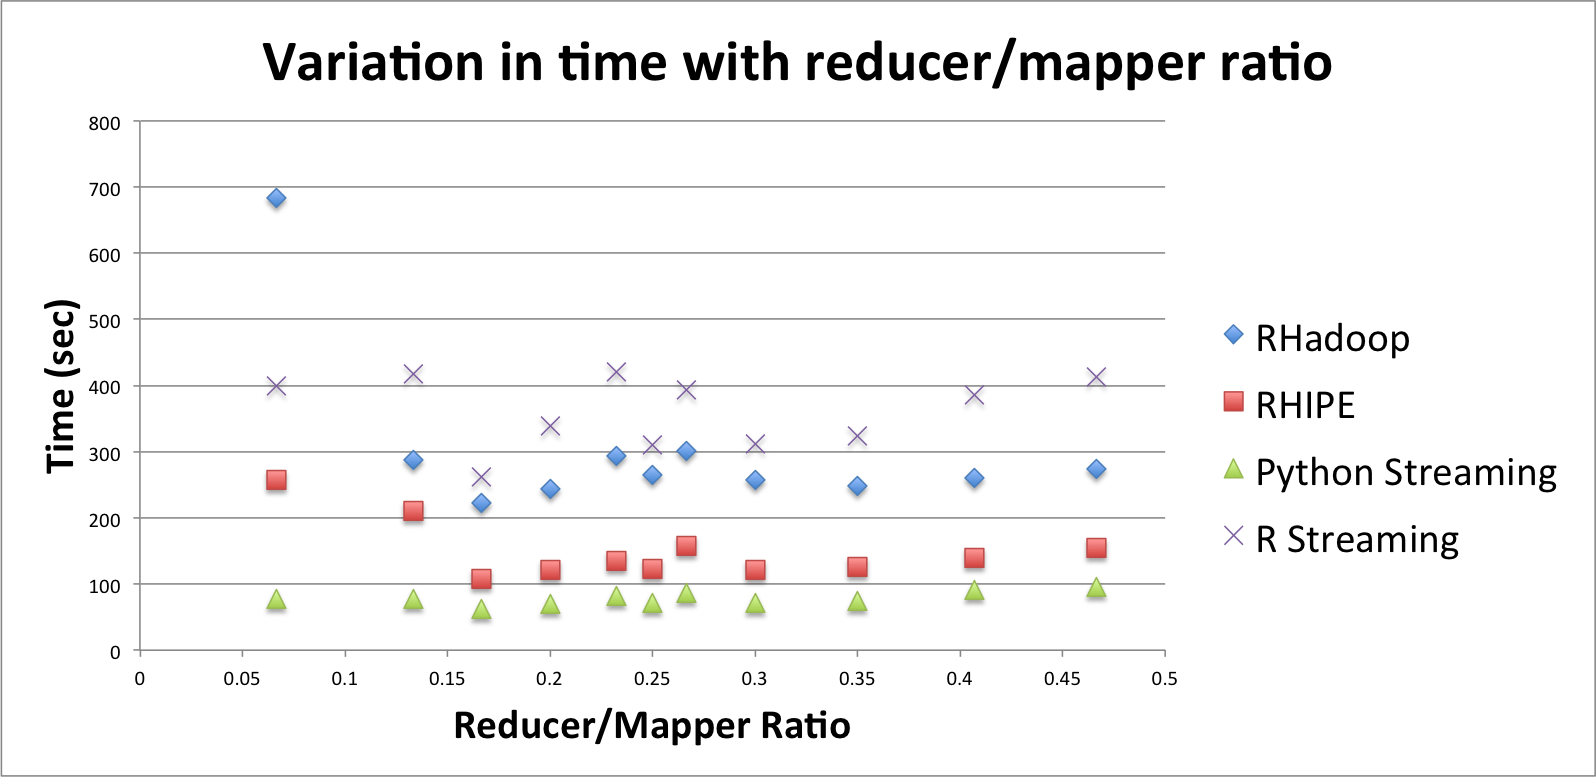
\includegraphics[width=16cm,height=10cm,keepaspectratio]{rm_ratio.png}

  \caption{Shows the variation of time to complete the job with respect to the reducer-mapper ratio.}

  \label{rm_ratio}

\end{figure}
The above figure shows the comparative performance of the four packages. We can order them with regards to performance as Python Streaming, RHIPE, RHadoop and R Streaming. Thus, the use of other packages as opposed to the simple to install and use R Streaming does give us a performance advantage. It can also be seen that 120 mappers and 20 reducers (a reducer to mapper ratio of 0.17) consistently had the lowest time for all the four methods. 

\subsubsection{Code Optimization}
\begin{figure}[!htb]
\minipage{0.5\textwidth}
  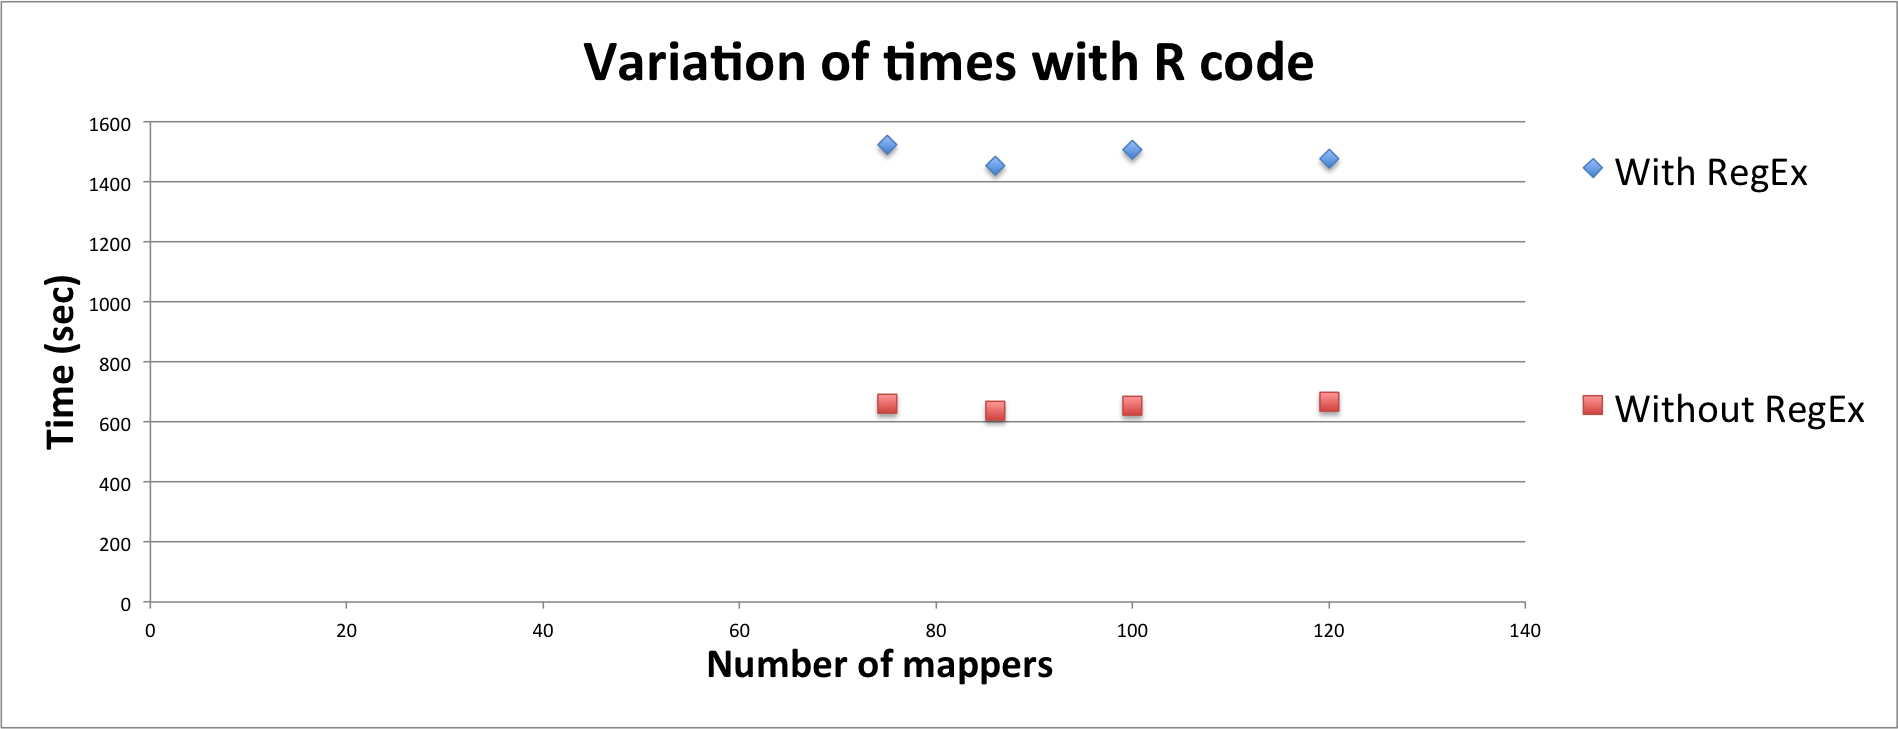
\includegraphics[width=\linewidth]{Regex_mappers.png}
  \caption{Performance impacts of regular expressions: with variation in the number of mappers}\label{fig:Regex_mappers}
\endminipage\hfill
\minipage{0.5\textwidth}
  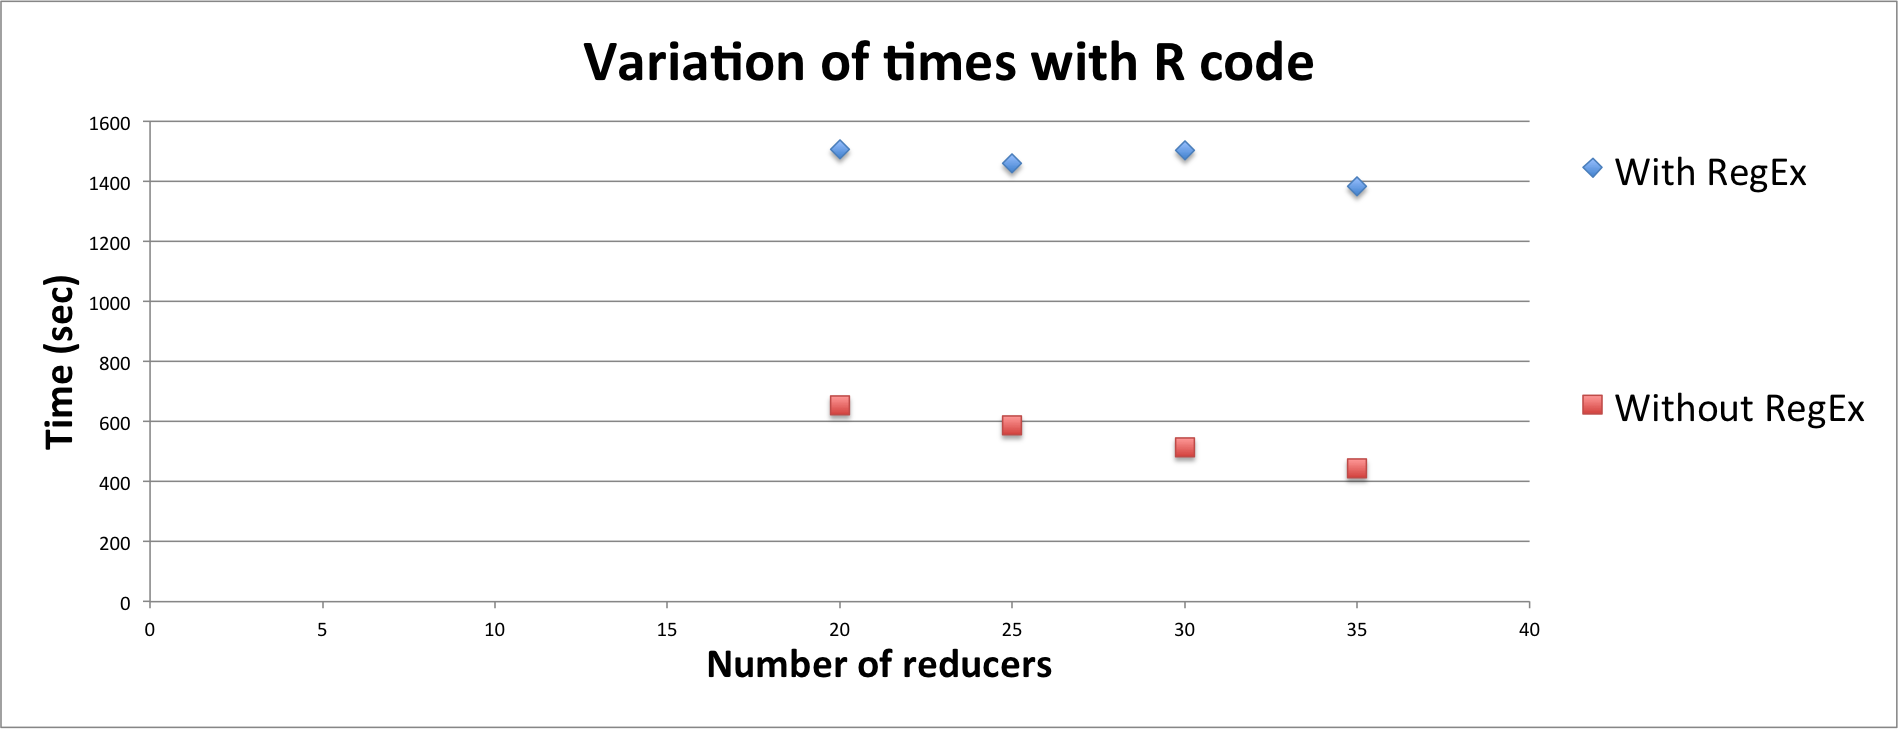
\includegraphics[width=\linewidth]{RegEx_reducers.png}
  \caption{Performance impacts of regular expressions: with variation in the number of reducers}\label{fig:RegEx_reducers}
\endminipage\hfill

\end{figure}
The graphs shows the drastic improvement in performance that resulted from using fixed string searches instead of regular expressions for parsing the input. We can see that just this small change led to a reduction in time of more than 50\%. This improvement was consistent over changes in number of mappers and reducers. 

\subsection{Results for Scalability tests}
We have found RHIPE to be very reliable with the minimum additional configuration compared to RHadoop and R Streaming which frequently failed on larger files. 

\begin{figure}

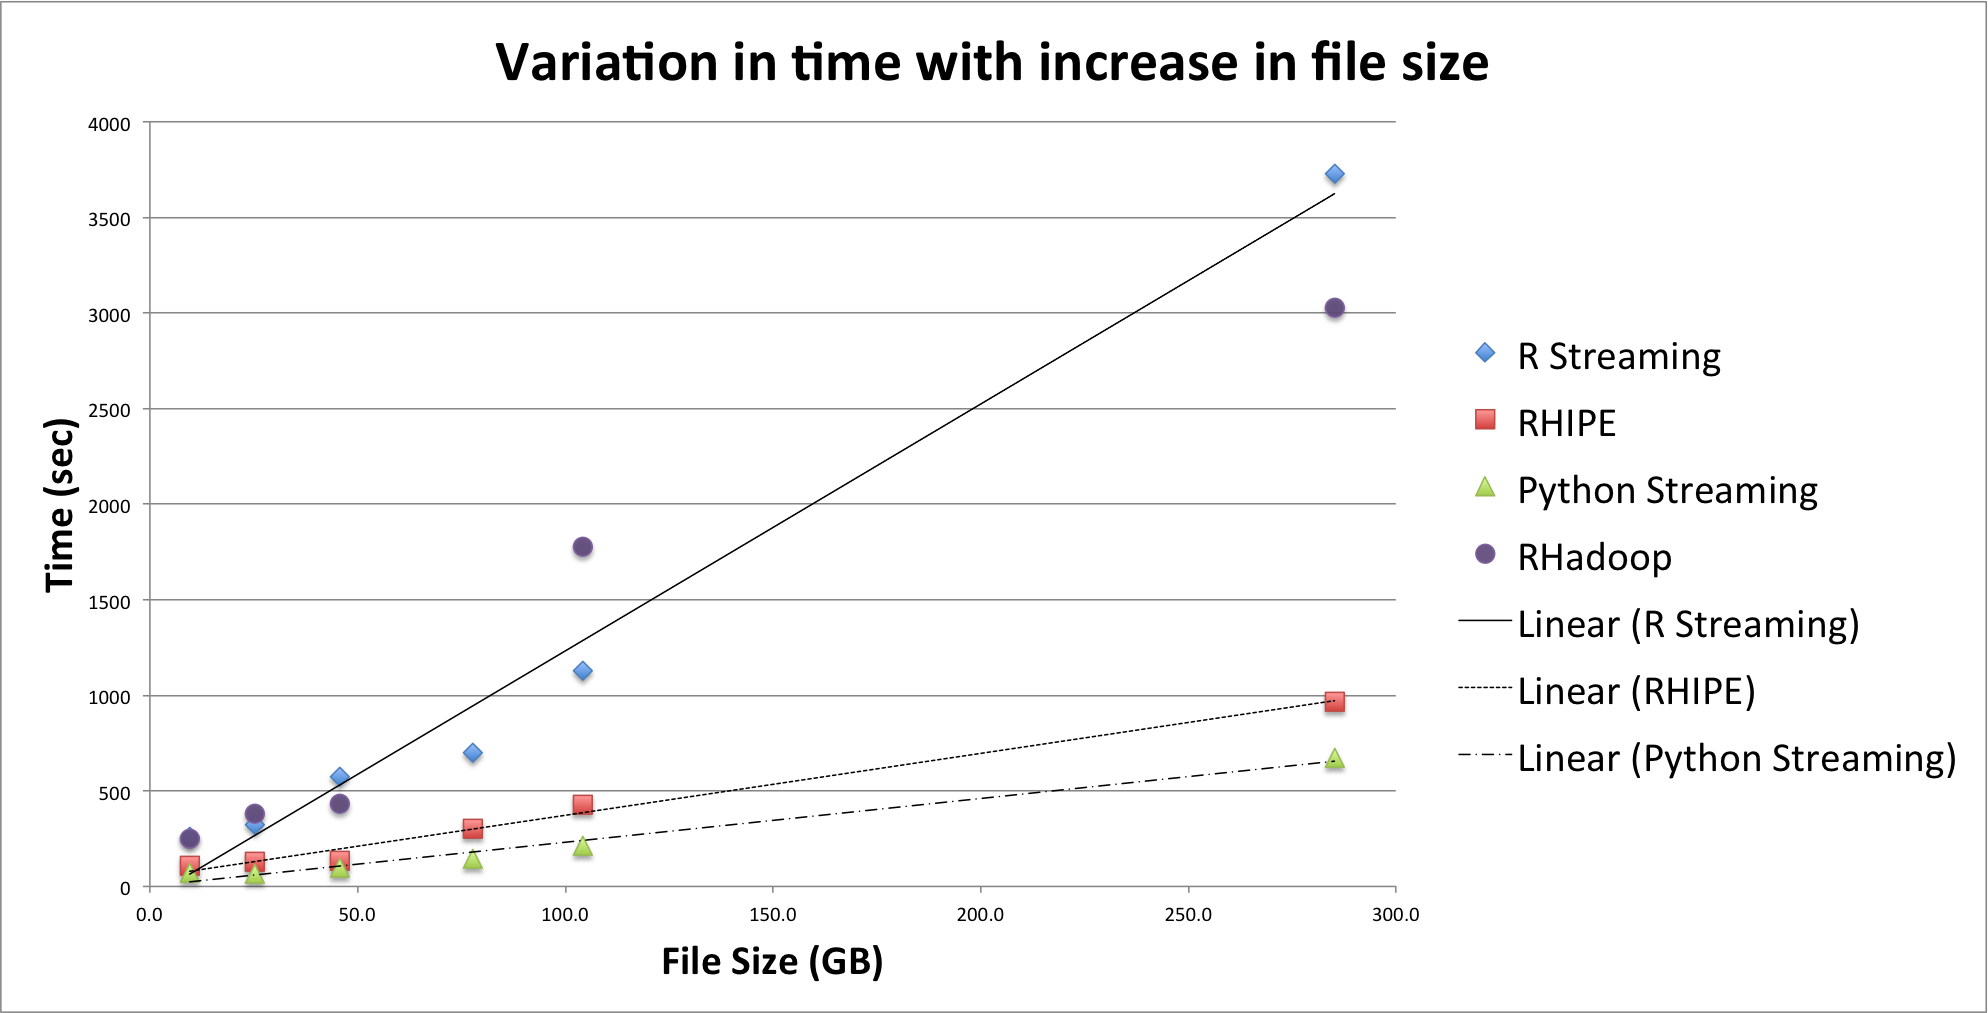
\includegraphics[width=16cm,height=10cm,keepaspectratio]{scaling.png}

  \caption{Shows the scalability of RHIPE, R Streaming and Python Streaming.}

  \label{scaling}

\end{figure}
It can be seen from the graph that R Streaming, RHadoop and RHIPE all scale linearly with an increase in workload for the \textit{worcount} application. However, RHadoop proved to be highly inconsistent since it failed a large proportion of the tests even for the cases it sometimes succeeded on. 

\subsection{Results for Large tests}
Large tests were only performed on the methods that successfully completed the Scalability tests. Which were RHIPE and Python. 

\begin{table}[H]
\begin{tabular}{ l|  l | l | l | l }
Size &\# Mappers & \# Reducers & RHIPE & Python \\ \hline
390GB & 5058 & 843 & 31mins, 0sec & 20mins, 10sec \\\hline
390GB & 6316 & 843 & 29mins, 59sec & 18mins, 40sec\\\hline
800GB & 17621 & 843 & 40mins, 10sec & 28mins, 25sec \\\hline
800GB & 17621 & 1000 & 1hr, 23mins, 8sec & 45mins, 0sec \\\hline
800GB & 17621 & 2848 & 2hr, 0min, 15sec & 1hr, 15min, 10sec \\\hline
\end{tabular}
\end{table}

The above table demonstrates when resources are strained, requesting more mappers or reducers, doesn't increase performance. The testing cluster's 64 nodes topped at about 750 active containers, in this case requesting 1000 reducers forced 250 to sit idle. Running the large tests we expected memory problems to arise, similar to what RHadoop and R Streaming both encountered in the previous test. However, both RHIPE and Python Streaming performed very well, maintained linearity, and finished without problems. 

\section{Best Practice Recommendation}
We have noticed a couple of improvements that should be kept in mind when developing R related Hadoop applications. A significant time reduction can be achieved by replacing regular expressions with fixed characters, in our simple \textit{wordcount} experiments processing time decreased by approximately 45\% even after mapper and reducer optimization was achieved.

Increasing the number of mappers and reducers doesn’t always increase performance and beyond the optimal ratio the time becomes minimally impacted. The continual increase of either mappers or reducers eventually leads to performance degradation. 

For RHadoop and Hadoop Streaming we can directly specify the mapper and reducer counts using \textit{mapreduce.job.maps} or \textit{mapreduce.job.reduces} parameters. To specify the number of mappers in RHIPE we specify the \textbf{chunk size} in bytes using \textit{mapred.max.split.size}. 
\begin{equation}
fileSize / chunkSize * 1024 * 1024 = NumMappers \nonumber
\end{equation}

 By default the number of mappers is chosen by the HDFS number of blocks, with the default \textbf{block-size} being 64MB and in production 128MB.  Given this a 1GB file will be stored in 8 blocks, and given 8 mappers. However in RHIPE specifying \textit{mapred.max.split.size} to 64MB will give us 16 mappers.  The same can be accomplished in Streaming by specifying \textit{mapreduce.job.maps=16}, however the block-size is the upper bound for chunk size. Hence, we cannot request less than 8 mappers or request the chunk-size to be more than 128MB. 
\begin{equation}
NumSplits \propto \frac{1}{chunkSize} \nonumber
\end{equation}

Comparing Python streaming times to RHIPE, RHadoop, and R Streaming we can conclude that R I/O can be very slow when done line at a time as streaming does by default. Depicted by the slow RHadoop and R Streaming times. RHIPE taking a different approach reads chunks at a time, with speeds closer to Python streaming implying lower I/O overhead. By supplying a custom InputFormat to the Hadoop streaming jar we should be able to achieve comparable speeds. 

In RHIPE testing the map and reduce functions does not have to be a cryptic guessing game. We can simulate a mapper using: 

\begin{lstlisting}[language=R]
data<-list(list(1,"Hello World"),list(2,"Long horn"))
map.keys<-lapply(data,"[[",1)
map.values<-lapply(data,"[[",2)

wordcount= function(map.keys, map.values){
  keys <- unlist(strsplit(unlist(map.values), split=' '))
  value <- 1
  lapply(keys, FUN=paste, value=value)
}

wordcount(map.keys,map.values)
\end{lstlisting}

We create the list (\textbf{Line 1}) required to pass to the RHIPE \textit{rhwatch} function, and split it into the key value pairs the mapper function will receive. Then create a function with a key, value signature \textbf{Line 5} that will process the data.  

In more general command line environment, Hadoop Streaming functionality can be tested using the following sequence of commands. 

\begin{lstlisting}[language=bash]
 $ cat book.txt | ./mapper.R | sort k1,1 | ./reducer.R
 
\end{lstlisting}

\section{Conclusion}
The \textit{wordcount} testing concluded RHIPE to be the preferred way of integrating R with Hadoop. Yet, when compared to Python we have discovered weaknesses in R itself, especially when many I/O operations are performed. Python constantly outmaneuvered R by approximately 35\% and failed in extremely few cases. While Python might be more efficient, R is more convenient for scientific purposes. 
With the choice of R, RHIPE consistently had a 35\% better performance as compared to RHadoop and R Streaming.

Though \textit{Wordcount} might not be an all encompassing benchmark, it is a good starting point for performance modeling of R and Hadoop integrations.


\acknowledgement
We sincerely appreciate Dr. Weijia Xu for mentoring us throughout the semester and Ruizhu Huang for valuable tips on the topic. 


\bibliography{references}
\clearpage

\section{Appendix}
\subsection{Code Used}
These are the mapper and reducer functions used in the\textit{wordcount}testing.

\subsubsection{Python Streaming}
\begin{lstlisting}[caption=Mapper.py]
#!/usr/bin/env python
import sys

# input comes from STDIN (standard input)
for line in sys.stdin:
    # remove leading and trailing whitespace
    line = line.strip()
    # split the line into words
    words = line.split()
    # increase counters
    for word in words:
        # write the results to STDOUT (standard output);
        # what we output here will be the input for the
        # Reduce step, i.e. the input for reducer.py
        #
        # tab-delimited; the trivial word count is 1
        print '%s\t%s' % (word, 1)
        
\end{lstlisting}


\begin{lstlisting}[caption=Reducer.py]
#!/usr/bin/env python

from operator import itemgetter
import sys

current_word = None
current_count = 0
word = None

# input comes from STDIN
for line in sys.stdin:
    # remove leading and trailing whitespace
    line = line.strip()

    # parse the input we got from mapper.py
    word, count = line.split('\t', 1)

    # convert count (currently a string) to int
    try:
        count = int(count)
    except ValueError:
        # count was not a number, so silently
        # ignore/discard this line
        continue

    # this IF-switch only works because Hadoop sorts map output
    # by key (here: word) before it is passed to the reducer
    if current_word == word:
        current_count += count
    else:
        if current_word:
            # write result to STDOUT
            print '%s\t%s' % (current_word, current_count)
        current_count = count
        current_word = word

# do not forget to output the last word if needed!
if current_word == word:
    print '%s\t%s' % (current_word, current_count)
\end{lstlisting}

\subsubsection{R Streaming}
\begin{lstlisting}[caption=Mapper.R]
#!/usr/bin/env Rscript
#https://github.com/glennklockwood/paraR

options(warn=-1)

outputCount= function(key, value) {
    cat(key,'\t',value,'\n',sep='')
}

stdin <- file('stdin', open='r')

while ( length(line <- readLines(stdin, n=1, warn=FALSE)) > 0 ) {
    #line <- gsub('(^\\s+|\\s+$)', '', line)
    keys <- unlist(strsplit(line, split=' ',fixed=TRUE))
    value <- 1
    lapply(keys, FUN=outputCount, value=value)
}
close(stdin)

\end{lstlisting}

\begin{lstlisting}[caption=Reducer.R]
#!/usr/bin/env Rscript
#https://github.com/glennklockwood/paraR
options(warn=-1)

last_key <- ""
running_total <- 0
stdin <- file('stdin','r')

outputCount <- function(word,count){
            cat(last_key,'\t',running_total,'\n',sep='')
}


while ( length(line <- readLines(stdin, n=1 , warn=FALSE)) > 0 ) {
    keyvalue <- unlist(strsplit(line, split='\t', fixed=TRUE))
    this_key <- keyvalue[[1]]
    value <- as.numeric(keyvalue[[2]])

    if ( identical(last_key,this_key) ) {
        running_total <- running_total + value
    }
    else {
        if ( !identical(last_key,"") ) {
	  outputCount(last_key,value)
	}
        running_total <- value
        last_key <- this_key
    }
}

outputCount(last_key,running_total)
close(stdin)
\end{lstlisting}



\subsubsection{RHadoop}

\begin{lstlisting}[caption=RHadoop mapper /reducer functions]
#!/usr/bin/env Rscript
library(rmr2)

bp =
  list(
    hadoop =
       list(
        D = paste("mapred.job.name=","RHadoop_wordcount", sep=''),
        D = paste("mapreduce.job.maps=",  "10", sep=''),
        D = paste("mapred.reduce.tasks=", "5", sep='')
          ))

rmr.options(backend.parameters = bp)
rmr.options("backend.parameters")

wordcount = 
    function(input, output = NULL, pattern = " "){
        wc.map = function(., lines) {
            keyval(unlist(strsplit(
               x = lines,
               split = pattern, fixed = TRUE)),1)}

 	    wc.reduce = function(word, counts ) {
	        keyval(word, sum(counts))}
 
        wc.vectorized.reduce = 
            function(k,vv) {
                vv = split(vv, as.data.frame(k), drop = TRUE)
                keyval(names(vv), vsum(vv))}
	      
      
          mapreduce(
            input = input,
            output = output,
            input.format = "text",
            map = wc.map,
            #reduce = wc.reduce, // when vectorized.reduce = F
            reduce = wc.vectorized.reduce, 
            vectorized.reduce = TRUE,
            in.memory.combine = TRUE,
            combine = TRUE
 )}
 
wordcount("hdfs:///sample.txt")
\end{lstlisting}

\subsubsection{RHIPE}
\begin{lstlisting}[caption=RHIPE mapper/reducer functions]
#!/usr/bin/env Rscript
library(Rhipe)

rhinit()
rhoptions(runner = 'sh /home/dotcz12/R/lib64/R/library/Rhipe/bin/RhipeMapReduce.sh')

mapred = list(
              mapred.max.split.size=as.integer(1024*1024*num_mappers),
              mapreduce.job.reduces=num_reducers #CDH3,4
            )
            
mapper <- expression( {
    keys <- unlist(strsplit(unlist(map.values), split=" "))
    value <- 1
    lapply(keys, FUN=rhcollect, value=value)
} )

reducer <- expression(
    pre = {
        running_total <- 0
    },
    reduce = {
        running_total <- sum(running_total, unlist(reduce.values))
    },
    post = {
         rhcollect(reduce.key, running_total)
    }
)
    
rhipe.results <- rhwatch(
                    map=mapper, reduce=reducer,
                    input=rhfmt("hdfs:///sample.txt", type="text"),
                    output="hdfs:///output_sample",
                    jobname="rhipe-wordcount",
                    mapred=mapred,
                    combiner=TRUE)

\end{lstlisting}


\end{document}

In general we have found Hadoop Streaming to be very efficient, the only drawback being the language of choice.

The amount of data used in applications has been increasing rapidly; R users in the scientific community are attempting to use R with large files. Our aim was to explore the different packages that can be used with R to facilitate big data analysis. We found three ways of combining R with Hadoop: RHadoop, RHIPE, and Hadoop Streaming. We examined the performance of these packages on a common big data program \textit{ wordcount}. We expected the slow I/O of R to be a performance bottleneck for this test, yet expected all three methods to be scalable. We deduced the optimal settings for relatively small files, did a scalability analysis with those settings, and checked the performance for larger files. We found RHIPE to be the most efficient choice amongst the three R alternatives and RHadoop frequently failed on large files.
RHIPE performed best amongst the R alternatives in our\textit{wordcount}testing and required minimal configuration. We discovered that small changes in R code can lead to considerable performance benefits. For instance, replacing regular expressions with fixed searches resulted in a 40\% speed up.